\documentclass{beamer}

\usepackage{graphics}
\usepackage{listings}

\usetheme{Bergen}
\usecolortheme{albatross}

\title{This is my presentation}
\author{My Name}
\date{Today 2010}

\begin{document}
\maketitle

\begin{frame}
   \frametitle{My First Slide}
   This is some heading text.
   \begin{itemize}
      \item This is the first point.
      \item This is the second point.
      \item This is the third point.
   \end{itemize}
   This is some ending text.
\end{frame}

\begin{frame}
   \frametitle{My Table Slide}
   This is a table. \\
   \begin{tabular}{|c|c|c|}
      \hline
      cell 1 & cell 2 & cell 3 \\
      \hline
      cell 4 & cell 5 & cell 6 \\
      \hline
   \end{tabular}
\end{frame}

\begin{frame}
   \frametitle{My Image Slide}
   This is where we look at an image of an earlier slide.
   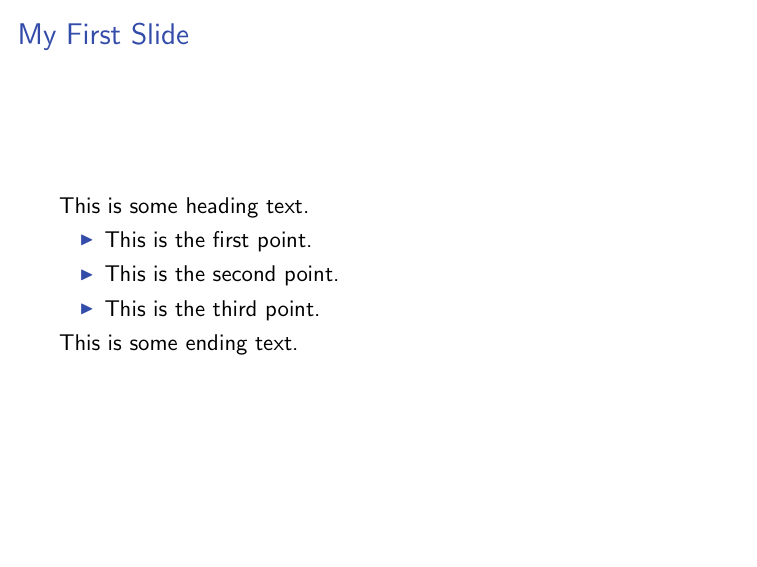
\includegraphics[angle=180,scale=0.5]{slide1.png}
\end{frame}

\begin{frame}[fragile,shrink=5]
   \frametitle{Sample Code}
   \begin{lstlisting}{language=C}
int main(int argc, char **argv) {
   int i=10;
   printf("Hello World!\n'');
   printf("The value of i is %d\n", i);
}
   \end{lstlisting}
\end{frame}

\end{document}

